% !TeX program = xelatex
% IEEE conference-format research proposal.
\RequirePackage[T1]{fontenc}
\documentclass[conference]{IEEEtran}

\usepackage{fontspec}
% Times/Helvetica/Courier-compatible fonts available in TeX Live and Overleaf.
\setmainfont{TeX Gyre Termes}
\setsansfont{TeX Gyre Heros}
\setmonofont{TeX Gyre Cursor}
\usepackage{cite}
\usepackage{amsmath,amssymb}
\usepackage{booktabs}
\usepackage{graphicx}
\usepackage{balance}
\usepackage{xurl}
\usepackage[hidelinks]{hyperref}
\urlstyle{tt}
\hypersetup{pdfauthor={Yu Zhang}}

\title{Evaluating C/C++ Vulnerability Detection with Independent Functions and Vulnerable--Fixed Pairs}
\author{
\IEEEauthorblockN{Yu Zhang}
\IEEEauthorblockA{ShanghaiTech University\\
Shanghai, China\\
\href{mailto:Zhangyu12026@shanghaitech.edu.cn}{Zhangyu12026@shanghaitech.edu.cn}}
}

\begin{document}
\maketitle

\begin{abstract}
This proposal investigates function-level vulnerability detection and discrimination between vulnerable code and its fixed version. Two evaluation subsets are constructed from local SecVulEval data. The first contains 200 functions: 160 labeled vulnerable and 40 labeled non-vulnerable, without annotated vulnerable--fixed relationships among selected functions. The second contains 200 vulnerable--fixed pairs, corresponding to 400 function records. Pairing follows explicit repair references. The subsets share neither source-record identifiers nor project--commit groups, yielding 600 distinct records. This proposal defines the research questions, sampling constraints, reproducibility information, and validity considerations. Experimental methods, models, and empirical results remain to be specified.
\end{abstract}

\begin{IEEEkeywords}
vulnerability detection, C/C++, paired evaluation, datasets
\end{IEEEkeywords}

\section{Introduction}
Vulnerability detection evaluation should establish whether a detector recognizes vulnerable functions while avoiding false alarms. It should also examine whether decisions change appropriately after a vulnerability is fixed. These questions motivate complementary evaluation units: individual functions and explicitly linked vulnerable--fixed pairs.

Published at AIware 2026, SecVulEval provides C/C++ functions with statement-level change annotations and contextual metadata~\cite{ahmed2026secvuleval}. PrimeVul emphasizes dataset quality, contamination control, and evaluation using vulnerable code and its patch~\cite{ding2025primevul}. Motivated by these studies, we propose a reproducible evaluation design using the local SecVulEval snapshot.

The independent subset evaluates functions without their annotated repair counterparts present. The paired subset examines appropriate labeling of both versions. Separating these cases can expose behavior obscured by aggregate results. Here, \emph{independent} describes sampling and repair-link constraints, not statistical independence.

\section{Research Objectives and Questions}
The objective is a traceable evaluation foundation for function-level detection and repair-sensitive discrimination:

\begin{enumerate}
    \item \textbf{RQ1: Function-level detection.} How effectively can a detector identify vulnerable functions and reject non-vulnerable functions on the independent subset with its prescribed 160:40 label composition?
    \item \textbf{RQ2: Vulnerable--fixed discrimination.} Can the detector identify the vulnerable version while recognizing the corresponding version as non-vulnerable according to the dataset labels?
    \item \textbf{RQ3: Complementarity of the subsets.} What differences in detector behavior emerge between independent functions and linked versions of the same function?
\end{enumerate}

Both subsets are evaluation resources; they do not define a training--test split. Training, tuning, and development data require separate specification. Detector effectiveness will be assessed only after the protocol and models are finalized.

\section{Dataset Construction}
\subsection{Source and Record Validation}
The source is the local SecVulEval workbook~\cite{ahmed2026secvuleval,secvulevaldata}. Its \texttt{train} worksheet contains 25,440 functions: 10,998 labeled vulnerable and 14,442 labeled non-vulnerable. These counts describe the local artifact.

Validation covers identifiers, labels, required text, and serialized lists. Seven records with unparseable \path{changed_statements} are excluded, leaving 25,433 usable records; metadata preserves their identifiers and exclusion reasons. Missing or excluded repair targets and pairs with identical trimmed function bodies are ineligible. The checks yield 10,004 candidate pairs.

\begin{figure*}[t]
\centering
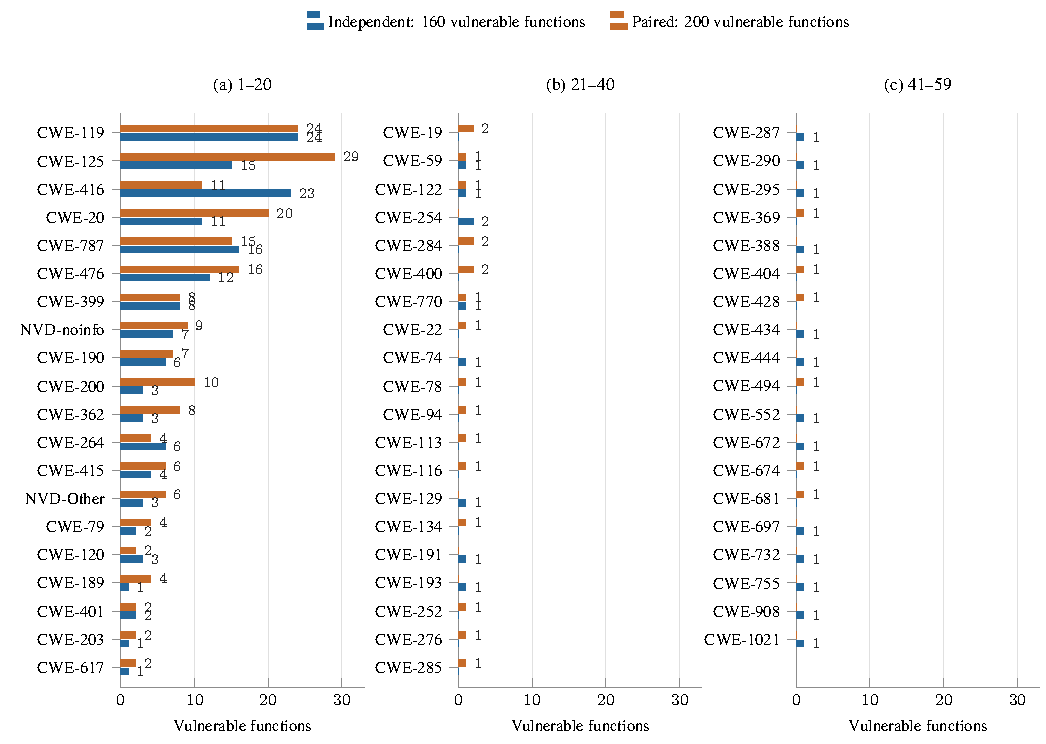
\includegraphics[width=\textwidth]{figures/cwe_distribution_en.pdf}
\caption{Counts of vulnerable functions by normalized CWE label. All 57 observed numeric CWE types and both NVD placeholder categories are shown, ordered by combined frequency across the three panels; every panel uses the same horizontal scale. NVD-noinfo and NVD-Other abbreviate NVD-CWE-noinfo and NVD-CWE-Other, respectively, and are metadata categories rather than specific weaknesses. Zero-count bars have no value label. Each vulnerable--fixed pair contributes only its vulnerable version.}
\label{fig:cwe-distribution}
\end{figure*}

\subsection{Subset A: Independent Functions}
Let the independent subset be
\begin{equation}
\mathcal{D}_{\mathrm{ind}}=\{(x_i,y_i)\}_{i=1}^{200},
\qquad y_i\in\{0,1\},
\end{equation}
where $x_i$ is a function record and $y_i=1$ denotes the vulnerable label. The subset contains exactly 160 vulnerable and 40 non-vulnerable functions. Its sampling constraints are:
\begin{enumerate}
    \item At most one function is selected from each \texttt{(project, commit\_id)} group.
    \item No selected vulnerable function has its annotated fixed counterpart in this subset.
    \item The 40 non-vulnerable records are not repair targets referenced by any vulnerable row in the source workbook.
\end{enumerate}
These constraints exclude annotated repair relationships among selected examples; they do not establish the absence of every relationship in upstream Git history.

\subsection{Subset B: Vulnerable--Fixed Pairs}
The paired subset is
\begin{equation}
\mathcal{D}_{\mathrm{pair}}=
\{(x_j^{v},x_j^{f})\}_{j=1}^{200},
\end{equation}
where $x_j^{v}$ is labeled vulnerable and $x_j^{f}$ is its corresponding fixed version labeled non-vulnerable. Each pair must satisfy the explicit reference
\begin{equation}
\texttt{fixed\_func\_idx}(x_j^{v})=\texttt{idx}(x_j^{f}).
\end{equation}
Both versions must share project, commit identifier, file path, and function name, with different trimmed function bodies. The shared commit identifier is an annotation-grouping key; \texttt{fixed\_func\_idx} establishes the version relationship. At most one pair is selected per project--commit group.

The 200 pairs comprise 400 function records. Correct labeling of both versions is the target; separate or joint presentation remains a protocol choice.

\begin{table}[t]
\caption{Composition of the Two Evaluation Subsets}
\label{tab:composition}
\centering
\begin{tabular}{@{}lcrrr@{}}
\toprule
Subset & Units & Vuln. & Non-vuln. & Functions\\
\midrule
$\mathcal{D}_{\mathrm{ind}}$ & 200 functions & 160 & 40 & 200\\
$\mathcal{D}_{\mathrm{pair}}$ & 200 pairs & 200 & 200 & 400\\
\bottomrule
\end{tabular}
\end{table}

\subsection{Sampling Order and Cross-Subset Isolation}
Sampling uses \texttt{random.Random(42)}. Shuffled eligible pairs are selected first, followed by 160 vulnerable and 40 eligible non-vulnerable functions, excluding previously used groups. Independent records are reshuffled before export. No project, CWE, or code-length quotas are imposed.

Let $I(\mathcal{D})$ denote the source-record identifiers in a subset and $G(\mathcal{D})$ its project--commit groups. Construction enforces
\begin{align}
I(\mathcal{D}_{\mathrm{ind}})\cap I(\mathcal{D}_{\mathrm{pair}})&=\varnothing,\\
G(\mathcal{D}_{\mathrm{ind}})\cap G(\mathcal{D}_{\mathrm{pair}})&=\varnothing.
\end{align}
The union contains 600 distinct records. Projects can overlap across different commits; this is not a project-disjoint split.

\subsection{Artifacts and Reproducibility}
The files \path{independent_200.json} and \path{vulnerable_fixed_200_pairs.json} store \texttt{samples} and \texttt{pairs}, respectively. Each pair contains \texttt{pair\_id}, \texttt{vulnerable}, and \texttt{fixed}. All 16 source fields and complete code are retained. Serialized lists become JSON arrays; \texttt{context} remains an unevaluated source string.

The generator \path{build_datasets.py} runs in Conda \texttt{pap} with Python 3.12.16, \texttt{openpyxl} 3.1.5, and \texttt{et\_xmlfile} 2.0.0. Metadata records the seed, source SHA-256, exclusions, and constraints. Source-field comparisons and seed-42 reproducibility have been verified. These are data-construction checks, not detection results.

\subsection{CWE Type Distribution}
Figure~\ref{fig:cwe-distribution} reports Common Weakness Enumeration (CWE) counts for the 160 independent vulnerable functions and the 200 vulnerable versions in the paired subset. The 40 independent negatives and 200 fixed counterparts are excluded. For this descriptive analysis, concatenated identifiers such as \texttt{CWE-125CWE-787} are split into individual CWE identifiers and deduplicated within each function; the source JSON files are unchanged. Each vulnerable subset covers 39 numeric CWE types, with 57 types in their union. Including the two NVD placeholder categories, the label-assignment totals are 173 and 213. These exceed function counts because some functions carry multiple CWE labels.

\balance
\section{Study Scope and Validity Considerations}
The independent subset deliberately contains 80\% vulnerable functions. This is an experimental composition and should not be interpreted as real-world vulnerability prevalence. The paired subset has balanced labels by construction. Aggregate outcomes across the two subsets would consequently require careful interpretation.

The study inherits source labels and repair links. A non-vulnerable label, or a successful repair of the annotated issue, does not prove that a function is free from every security defect. Project--commit separation controls one form of overlap, but does not guarantee the absence of similar code, shared vulnerability families, or pretraining contamination. No project-disjoint or chronological generalization claim is currently supported.

The small sample size and absence of CWE stratification limit coverage. Versions within a pair are related observations, so 400 paired records should not be treated as 400 unrelated evaluation units. Labels, repair references, commit messages, CVE identifiers, and change annotations will be retained for traceability; the future protocol must specify which fields are exposed as model inputs to avoid revealing the answer. Failure handling and any additional development split also remain to be defined.

\section{Expected Contributions}
The planned contributions are reproducible evaluation subsets and a traceable basis for distinguishing individual-function detection from vulnerable--fixed discrimination. Construction artifacts are available; model-performance conclusions await experimentation.

\section{Experimental Methods}
\label{sec:methods}
% Intentionally blank. Add the experimental protocol, inputs, metrics,
% failure handling and statistical analysis after the design is finalized.

\section{Experimental Models}
\label{sec:models}
% Intentionally blank. Add model identities, versions and configurations.

\section{Experimental Results}
\label{sec:results}
% Intentionally blank. Add only measured results and supporting analysis.

\bibliographystyle{IEEEtran}
\bibliography{references}
\end{document}
